\subsection{Methodology}

After the dataset creation ...

The end of each Karoo GP training produces a multivariate exression with heighest fitness score. We repeat the training process 200 times to get 200 expressions for each label (hasNS and hasRemnant). Due to the stochastic nature of the GP algorithm, the expressions mostly tend to be unique depending upon the complexity of the classification problem. Each expression can then be used to classify the reconstructed source parameters to determine the labels hasNS and hasRemnant by substituting the values in the expression. If the result is greater or equal to zero, we classify the reconsturcted set of prameter as true and false otherwise. The performace of each of the expressions against the testing set for one EoS is shown in Fig \ref{fig:FPR_TPR}. As seen in the plots, the average performace of hasRemnant expressions is better than hasNS expressions. Also the winning expressions are more dispersed in case of hasRemnant.  \textcolor{red}{Shall we explain the reasons: hasNS being simpler classification but contaminated by poor reconstructions by the pipeline. HasRemnant is more complex leading to more variable winning trees.} 
\linebreak
\textbf{Calculation of Probability:} Using testing set, we compute probabilities using bayesian method. HasNS and hasRemnant are not inherintly independent quantities since there can be no hasRemnant without hasNS. Hence, we utilize both hasNS winning expressions and hasRemnant winning expressions for quantifying probabilities $p(hasNS)$ and $p(hasRemnant)$. If XREM denotes the number of hasRemnant winning trees which classifies given set of parameter as true and XNS denotes the number of hasNS winning trees which classifies as true, we compute the probability on the testing set as:    

\begin{equation}
\begin{split}
p(HasNS| XREM \cap XNS) =\\ 
\frac{p(XREM \cap XNS|HasNS).p(HasNS)}{p(XREM \cap XNS)}
\end{split}
\end{equation}
\begin{equation}
\begin{split}
p(HasRemnant| XREM \cap XNS) =\\ 
\frac{p(XREM \cap XNS|HasRemnant).p(HasRemnant)}{p(XREM \cap XNS)}
\end{split}
\end{equation}

\begin{figure*}[htp]
  \centering
  \subfloat[]{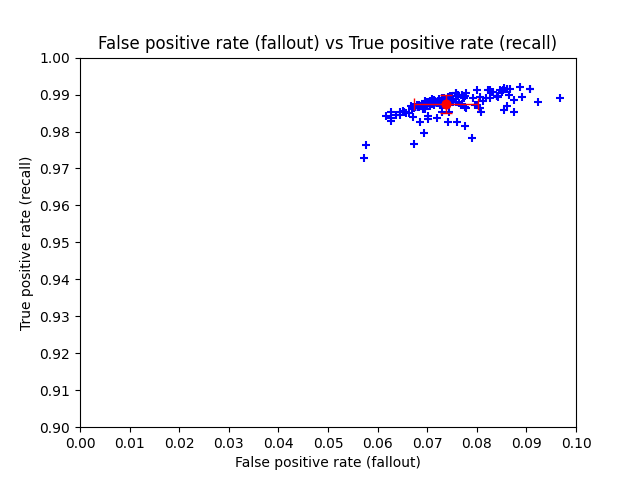
\includegraphics[scale=0.5]{plots/FPR_TPR/FPR_TPR_NS_MS1_PP.png}}\quad
  \subfloat[]{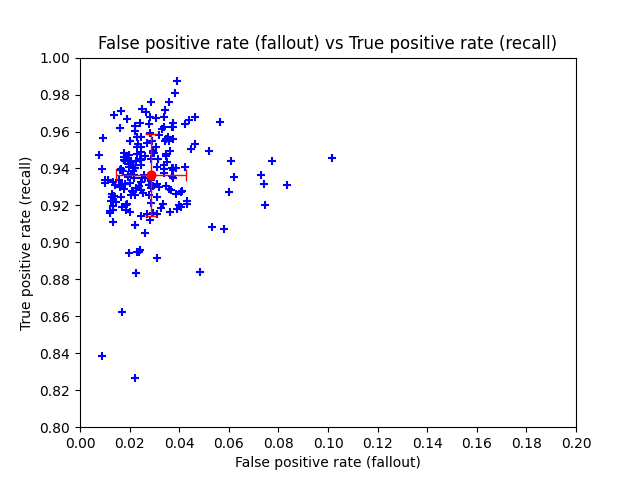
\includegraphics[scale=0.5]{plots/FPR_TPR/FPR_TPR_EMB_MS1_PP.png}}
  \caption{The plot on the left is a FPR (False Positive Rate) vs (True Positive Rate) plot for all 200 winning expressions for hasNS classification on MS1-PP EoS. The red dot is the average of TPR and FPR of the expressions and the vetricle and horizontal spread are the one sigma values for TPR and FPR respectively. The plot on the right is similar but for hasRemnant classification.  }
  \label{fig:FPR_TPR}
\end{figure*}

There as some caveats to this calculation. Given a finite testing set, we cannot fully compute the entire parameter space (201 x 201 cases) of the probability since there are some cases which are highly unlikely to occur, like $p(hasNS | XNS=0 \cap XREM=200)$. Also, our probability computations might also suffer due to the finite testing set size. The resulting probability distribution is highly rugged and \textcolor{red}{discontinuous or incomplete}. Hence, in order to span the entire parameter space of the probability, we use gasussian process regression (GPR). 

\textbf{Gaussian Process Regression:} We implement GPR using a python package gpytorch \cite{gpytorch}. Using the RQ




